\documentclass{article}
\usepackage{graphicx}
\usepackage{amsmath}
\usepackage{amssymb}
\usepackage{hyperref}
\usepackage{float}
\usepackage{tikz}
\usepackage{subcaption} % for subfigures

\title{CSC311 Project Final Report}
\author{Group Members: \\ Zixuan Zeng 1008533419 \\ ... \\ ...}

\begin{document}

\maketitle

Note: Contributions and LLM are at the end of this report.

\newpage
\vspace*{5cm}
\begin{center}
\Large\bfseries Part A
\end{center}
\newpage

\section*{Q1 - KNN}

\subsection*{1.(a)}

\begin{figure}[H]
    \centering
    \begin{subfigure}{0.45\textwidth}
        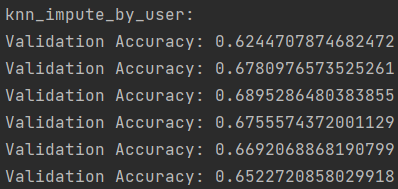
\includegraphics[width=\textwidth]{knn_impute_by_user_result.png}
    \end{subfigure}
    \hfill
    \begin{subfigure}{0.45\textwidth}
        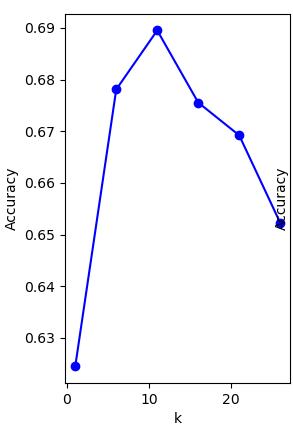
\includegraphics[width=\textwidth]{knn_impute_by_user_plot.png}
    \end{subfigure}
    \caption{Accuracy vs k for KNN Impute by User}
\end{figure}

\subsection*{1.(b)}

\begin{figure}[H]
    \centering
    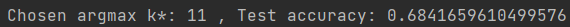
\includegraphics[width=\textwidth]{knn_impute_by_user_test.png}
    \caption{Test accuracy with k*}
\end{figure}

\subsection*{1.(c)}

The underlying assumption is that if question A is answered similarly by many students as question B, A’s predicted response from specific students matches that of question B.

\begin{figure}[H]
    \centering
    \begin{subfigure}{0.45\textwidth}
        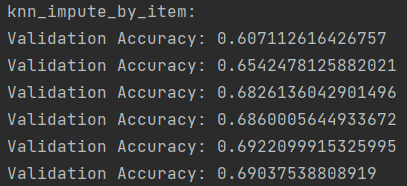
\includegraphics[width=\textwidth]{knn_impute_by_item_result.png}
    \end{subfigure}
    \hfill
    \begin{subfigure}{0.45\textwidth}
        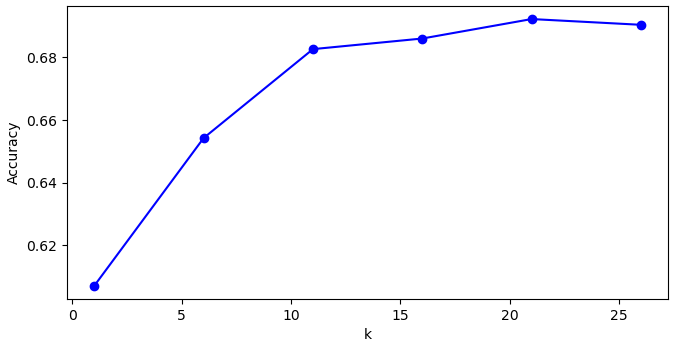
\includegraphics[width=\textwidth]{knn_impute_by_item_plot.png}
    \end{subfigure}
    \caption{Accuracy vs k for KNN Impute by Item}
\end{figure}

\begin{figure}[H]
    \centering
    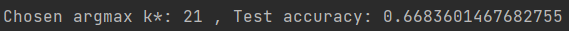
\includegraphics[width=\textwidth]{knn_impute_by_item_test.png}
    \caption{Test Accuracy with k*}
\end{figure}
\newpage

\subsection*{1.(d)}
The test accuracy for the user-based method (0.6842) is higher than that for the item-based method (0.6684). Therefore, the user-based collaborative filtering method performs better than the item-based collaborative filtering method in this case.

\subsection*{1.(e)}
\begin{itemize}
    \item Computationally expensive. KNN practically has no training process. With large datasets, as the number of students/questions grow, the time required to compute the distances and to identify the nearest neighbors at test time grows significantly.
    \item Curse of Dimensionality. When the sparse\_matrix has too many missing values, it’s hard to find good nearest neighbors, since most points will be about the same distances. This affects the prediction accuracy.
\end{itemize}
\newpage


\section*{Q2 - IRT}

\subsection*{2.(a)}

\[
p(c_{ij} = 1 | \theta_i, \beta_j) = \frac{\exp(\theta_i - \beta_j)}{1 + \exp(\theta_i - \beta_j)} = \sigma(\theta_i - \beta_j)
\]
log-likelihood:
\[
\log p(C | \theta, \beta) = \sum_{i}\sum_{j} \left[ c_{ij} (\theta_i - \beta_j) - \log (1 + \exp(\theta_i - \beta_j)) \right]
\]
The derivative of the log-likelihood with respect to $\theta_i$:
\[
\frac{\partial \log p(C | \theta, \beta)}{\partial \theta_i} = \sum_{j} \left[ c_{ij} - \sigma(\theta_i - \beta_j) \right]
\]
The derivative of the log-likelihood with respect to $\beta_j$:
\[
\frac{\partial \log p(C | \theta, \beta)}{\partial \beta_j} = \sum_{i} \left[ - c_{ij} + \sigma(\theta_i - \beta_j) \right]
\]

\subsection*{2.(b)}

\begin{figure}[H]
    \centering
    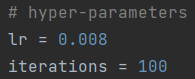
\includegraphics[width=0.3\textwidth]{2(b)1.png}
    \caption{Hyper-Parameters}
\end{figure}
\begin{figure}[H]
    \centering
    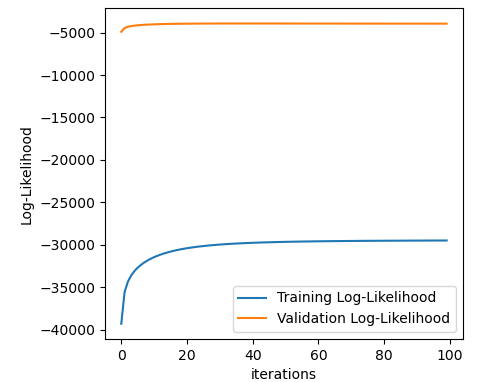
\includegraphics[width=0.65\textwidth]{2(b)2.png}
    \caption{Training and Validation Log-Likelihoods vs Iteration}
\end{figure}

\subsection*{2.(c)}
\begin{figure}[H]
    \centering
    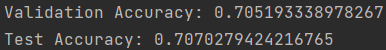
\includegraphics[width=0.6\textwidth]{2(c).png}
    \caption{Final Validation \& Test Accuracy}
\end{figure}

\subsection*{2.(d)}
The three curves are all in S shape, as the sigmoid function. They represent the probability of correct responses as a function of student ability $\theta$.\newline
It shows that students with a high ability have a high probability of answering correctly.\newline
Also, question with a high difficulty is skewed to the right, meaning it has a lower probability of being answered correctly.
\begin{figure}[H]
    \centering
    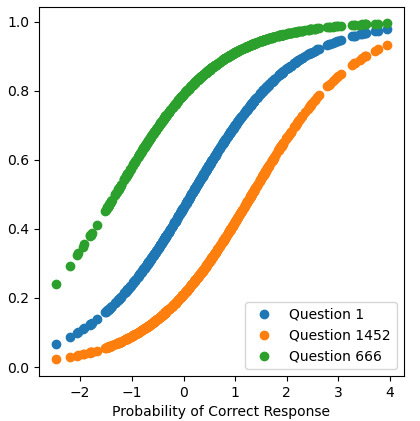
\includegraphics[width=0.6\textwidth]{2(d).png}
    \caption{Probability of Correct Response vs Theta}
\end{figure}
\newpage


\section*{Q3 - (i) Option 1: Matrix Factorization}

\subsection*{3(i).(a)}
\begin{figure}[H]
    \centering
    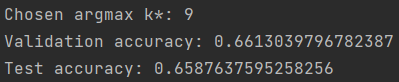
\includegraphics[width=0.7\textwidth]{3(i)(a).png}
    \caption{SVD: Final Validation \& Test Performance with chosen k\*}
\end{figure}

\subsection*{3(i).(b)}
Filling the missing values with averages or zeros does not accurately reflect the data's underlying structure. There will be loss or distorsion of information.

\subsection*{3(i).(c)(d)(e)}
\begin{figure}[H]
    \centering
    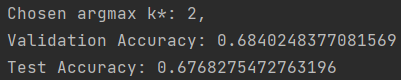
\includegraphics[width=0.7\textwidth]{3(i)(c)(d).png}
    \caption{ALS: Final Validation \& Test Performance with chosen k\*}
\end{figure}
\begin{figure}[H]
    \centering
    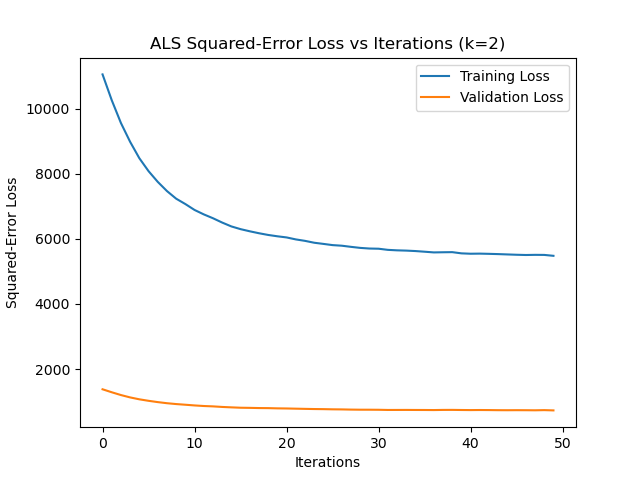
\includegraphics[width=0.8\textwidth]{3(i)(e).png}
    \caption{ALS: Squared-Error Loss vs Iterations}
\end{figure}
\newpage


\section*{Q4 - Ensemble}
Ensemble Process:
\begin{enumerate}
    \item For each separate model, create different subsets of the training data of the same size of the original training data by sampling with replacement. 
    \item Train KNN, IRT, ALS. Report validation accuracy of each model. Use the models to generate predictions for validation and test data.
    \item Using the three sets of predictions, calculate the mean of predictions.
    \item Evaluate the ensembled prediction for final ensembled validation and test accuracy.
\end{enumerate}
The ensemble does achieve better performance than individual models based on the final accuracy results. Because ensemble approach reduces the variance by combining the three models, which improved generalization.
\begin{figure}[H]
    \centering
    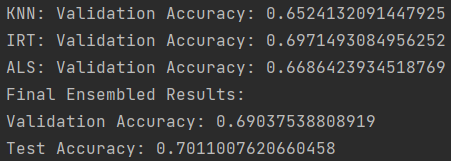
\includegraphics[width=0.7\textwidth]{4.png}
    \caption{Individual Model \& Final Ensemble Accuracies}
\end{figure}
\newpage


\vspace*{5cm}
\begin{center}
\Large\bfseries Part B
\end{center}
Note: This part consists of an ensemble of two models, created by two team members with separate algorithm analysis.
\newpage


\section*{Modified ALS - Zixuan Zeng}
\subsection*{Q1 - Formal Description:}
\begin{itemize}
    \item Base Model: Matrix Factorization with ALS\newline
    The base model of Matrix Factorization with ALS captures some nuanced properties of users and questions. \newline
    However, it initializes both matrices U and Z with values selected uniformly at random between 0 and $\frac{1}{np.sqrt(k)}$, for applying SGD to fit data into the model for the derivation of the k principal components.\newline
    The randomness in latent factor initialization can lead to poor prediction quality and convergence to local minima.\newline
    Also, This method lacks interpretability. Since we have no knowledge over the desired demensionality of PCA, along with the non-deterministic nature of the algorithm, the argmax k* fluctuates significantly. 
    \item Modified ALS:\newline
    My proposed modified model combines ALS with content-based approach to handle the existing problems.\newline
    It incorporates the question metadata, using the subjects of each question as additional factors.\newline
    Introduce new matrices: $U_s \in \mathbb{R}^{n\times subjects} $ and $Z_s \in \mathbb{R}^{m\times subjects} $, where U\_s is also initialized by sampling uniformly at random, but Z\_s is initialized to a sparse matrix with entries filled using question-subjects metadata, set at $\frac{1}{np.sqrt(num\_subjects)}$\newline

\end{itemize}
Prediction given by:
\[R_{ij} \approx U^T Z + U_s^T Z_s\]\newline
Squared Error Loss: 
\[L = \frac{1}{2} \sum_{(n,m) \in O} (C_{nm} - (U^T Z + U_s^T Z_s))^2\]
Update Rules for SGD:
\[U_i \leftarrow U_i - \alpha \frac{\partial L}{\partial U_i} = -(C_{ij} - (U^T Z + U_s^T Z_s)) Z_j\]
\[Z_j \leftarrow Z_j - \alpha \frac{\partial L}{\partial U_i} = -(C_{ij} - (U^T C + U_s^T Z_s)) U_i\]
\[U_{si} \leftarrow U_{si} - \alpha \frac{\partial L}{\partial U_{si}} = -(C_{ij} - (U^T Z + U_s^T Z_s)) Z_{sj}\]
\[Z_{sj} \leftarrow Z_{sj} - \alpha \frac{\partial L}{\partial Z_{sj}} = -(C_{ij} - (U^T Z + U_s^T Z_s)) U_{si}\]
\newpage

\subsection*{Q2 - Figure or Diagram:}
\begin{figure}[h!]
    \centering
    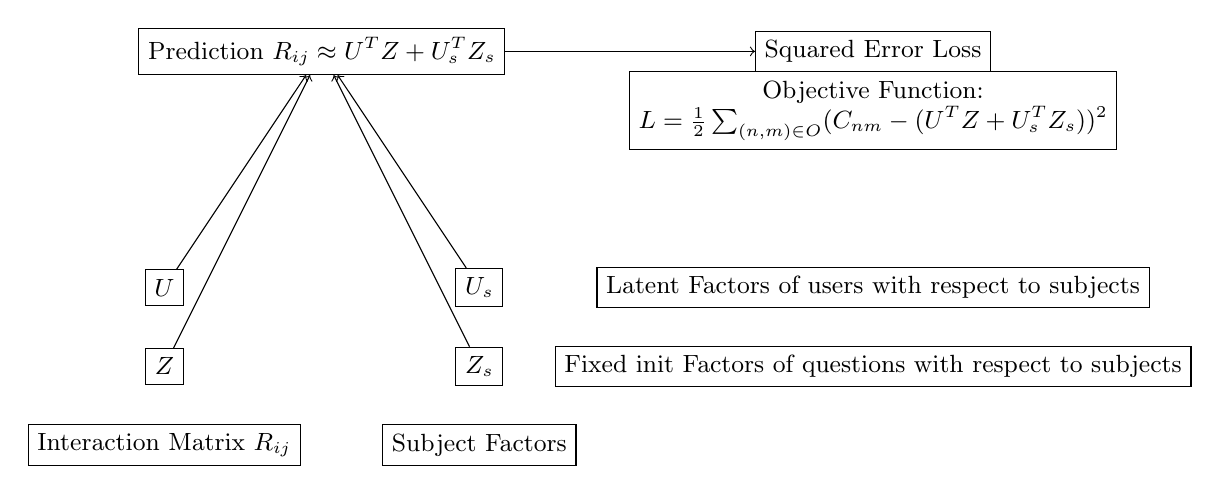
\begin{tikzpicture}[node distance=3cm, every node/.style={draw, font=\small, align=center}]
        % Nodes
        \node (Pred) [rectangle] {Prediction $R_{ij} \approx U^T Z + U_s^T Z_s$};
        \node (Loss) [rectangle, right of=Pred, xshift=4cm] {Squared Error Loss};
        \node (U) [rectangle, below of=Pred, xshift=-2cm] {$U$};
        \node (Z) [rectangle, below of=U, yshift=2cm] {$Z$};
        \node (Us) [rectangle, below of=Pred, xshift=2cm] {$U_s$};
        \node (Zs) [rectangle, below of=Us, yshift=2cm] {$Z_s$};

        % Arrows
        \draw[->] (U) -- (Pred);
        \draw[->] (Z) -- (Pred);
        \draw[->] (Us) -- (Pred);
        \draw[->] (Zs) -- (Pred);
        \draw[->] (Pred) -- (Loss);

        % Descriptions
        %\node [below of=R, yshift=-0.5cm] {Matrix Factorization with ALS};
        \node [right of=Us, xshift=2cm] {Latent Factors of users with respect to subjects};
        \node [right of=Zs, xshift=2cm] {Fixed init Factors of questions with respect to subjects};
        \node [below of=Z, yshift=2cm] {Interaction Matrix $R_{ij}$};
        \node [below of=Zs, yshift=2cm] {Subject Factors};
        \node [below of=Loss, yshift=2.25cm] {Objective Function: \\ $L = \frac{1}{2} \sum_{(n,m) \in O} (C_{nm} - (U^T Z + U_s^T Z_s))^2$};
    \end{tikzpicture}
    \caption{Diagram of the Modified ALS Model showing the interaction between matrices $U$ and $Z$, $U_s$ and $Z_s$, the prediction formula, and the squared error loss function.}
    \end{figure}

\subsection*{Q3 - Comparison / Demonstration:}
Proposed hypothesis:

The modified ALS improves prediction accuracy due to better optimization strategies: incorporating new metadata as factors that influence the predictions.

Since the new algorithm without this feature is just the base ALS model, we will just test against the base ALS model using separate argmax hyperparameters.

\begin{figure}[H]
    \centering
    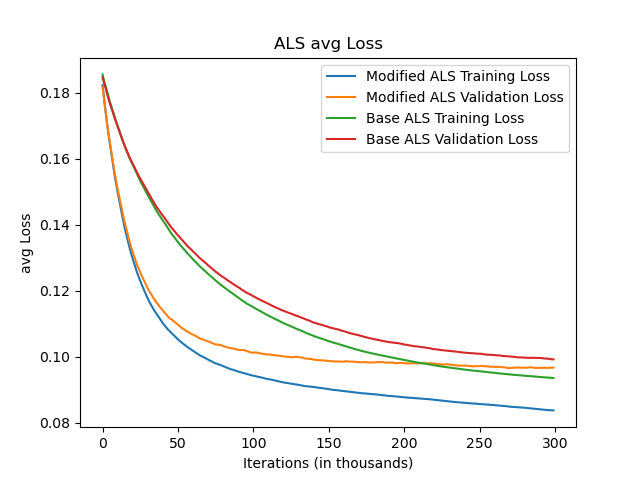
\includegraphics[width=0.6\textwidth]{bz1.png}
    \caption{Average Loss vs Iterations: Modified ALS vs Base ALS}
\end{figure}

\begin{figure}[H]
    \centering
    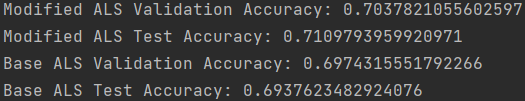
\includegraphics[width=0.7\textwidth]{bz2.png}
    \caption{Validation \& Test Accuracy: Modified ALS vs Base ALS}
\end{figure}
As seen in the plot, the modified ALS (as blue and yellow lines) has a lower squared loss error (averaged by len(train\_data)).

It also has better validation accuracy of 0.704 and test accuracy of 0.711, compared to the base ALS model's validation accuracy of 0.697 and test accuracy of 0.694.

Therefore the modified ALS does have a better optimization.

\subsection*{Q4 - Limitations:}
\begin{itemize}
    \item The modified model assumes that subject metadata and latent factors capture all relevant aspects of user-question interactions, which may not always be the case.
    \item The reason is that this model emphasizes on the importance and correct catagorization of subject metadata and correctness of turning user-question interactions into latent factors. This method overlooks other important factors such as student metadata, contexual info, etc\dots
    \item To extend the current implementation to mitigate these limitations, we could integrate additional features or context-aware factors into the model to capture more nuanced interactions.
\end{itemize}
\newpage


\section*{Hybrid KNN - Hao Liu}

\subsection*{Q1 - Formal Description:}
The Hybrid KNN model combines both user-based and item-based K-Nearest Neighbors (KNN) algorithms to improve the accuracy of predicting students' responses to diagnostic questions. Below is the detailed definition and methodology of the hybrid KNN model.

Formula Definition:
\begin{enumerate}
    \item User-based KNN Imputation:\newline
    Given a sparse matrix, where $x_{ij}$ represents the response of student i to question j (0 for incorrect, 1 for correct, and NaN for missing), we can use user\-based KNN to fill in the missing values. For each missing value $x_{ij}$, we find the k most similar students to student i and use their answers to fill in the missing value.
    Let $N\_i$ represent the k nearest neighbors of student i. The imputed value is calculated as:
    \[\hat{x}_{ij}^{user} = \frac{1}{k} \sum_{u \in N_i} x_{uj}\]
    \item Item-based KNN Imputation:\newline
    Similarly, we can use item-based KNN to fill in the missing values. For each missing value $x_{ij}$, we find the k most similar questions to question j and use their responses to fill in the missing value.
    Let $N\_i$ represent the k nearest neighbors of question j. The imputed value is calculated as:
    \[\hat{x}_{ij}^{item} = \frac{1}{k} \sum_{v \in N_j} x_{vj}\]
    \item Hybrid Imputation:\newline
    The final imputed value is a weighted combination of the user-based and item-based imputations:
    \[\hat{x}_{ij}^{hybrid} = \alpha\hat{x}_{ij}^{user} + (1-\alpha)\hat{x}_{ij}^{item}\]
    where $\alpha$ is a user-defined weight parameter to balance the user-based and item-based imputations.
\end{enumerate}
\newpage 

Algorithm Pseudocode:
\begin{figure}[H]
    \centering
    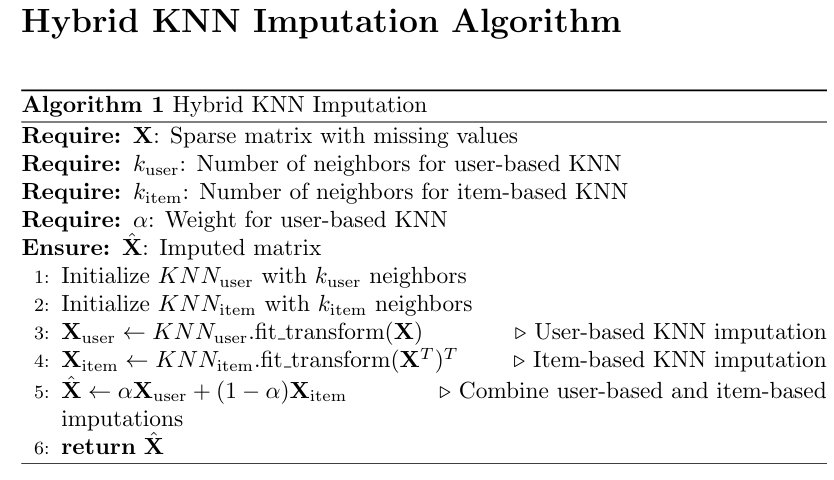
\includegraphics[width=0.85\textwidth]{bl1.png}
    \caption{Algorithm Pseudocode}
\end{figure}

\subsection*{Q2 - Figure or Diagram:}
The provided graph shows the validation accuracy of the hybrid KNN imputation algorithm as a function of the number of neighbors k. The analysis focuses on understanding the performance trends and determining the optimal k value for the hybrid KNN model.
\begin{figure}[H]
    \centering
    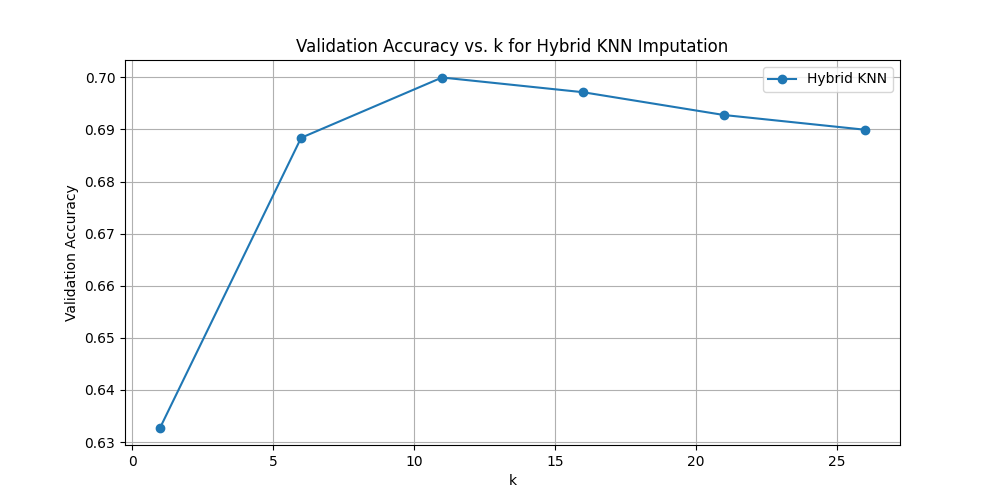
\includegraphics[width=0.85\textwidth]{bl2.png}
    \caption{Hybrid KNN Imputation Results}
\end{figure}
Observations:
\begin{enumerate}
    \item Accuracy Improvement with Increasing k:
    For small values of k (specifically k = 1), the validation accuracy is relatively low (approximately 0.63).
    As k increases from 1 to 11, there is a significant improvement in validation accuracy, reaching a peak of approximately 0.70 at k = 11.
    \item Optimal k:
    The highest validation accuracy is observed at k = 11. This indicates that using 11 neighbors provides the best balance between capturing sufficient information from similar users and items while avoiding overfitting to noise.
    \item Decreasing Accuracy for Larger k:
    After k = 11, the validation accuracy begins to decrease gradually. This decline suggests that using too many neighbors may introduce less relevant or noisy data, which negatively impacts the model's performance.
\end{enumerate}

\subsection*{Q3 - Comparison / Demonstration:}
Through experiments, we compared the validation accuracy and test accuracy of the hybrid KNN model with the baseline models (user-based KNN and item-based KNN). The comparison was performed using different values of k (number of neighbors) to evaluate the performance of each model. Below are the observations and analysis based on the results.
\begin{figure}[H]
    \centering
    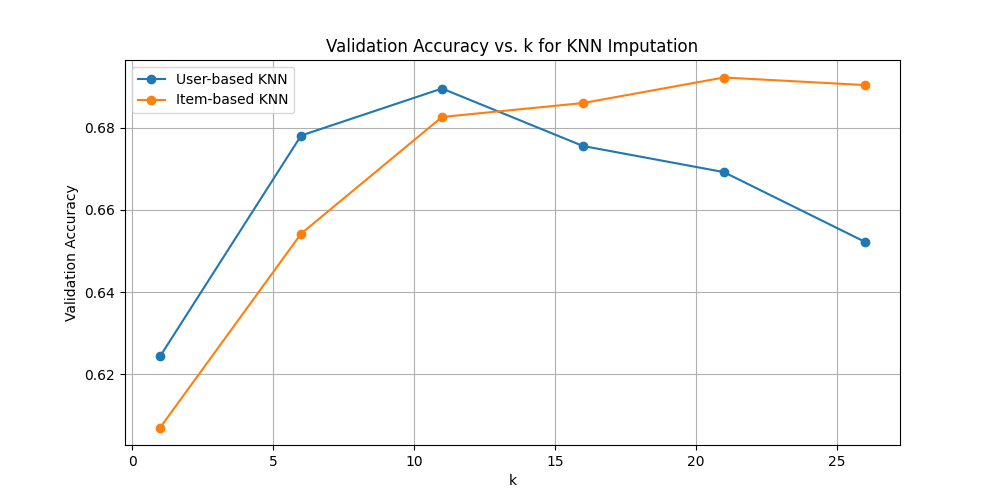
\includegraphics[width=0.85\textwidth]{bl3.png}
    \caption{Validation Accuracy vs k for KNN Imputation}
\end{figure}

\begin{enumerate}
    \item Comparison of Validation accuracy\newline
    The graph shows the validation accuracy for user-based KNN and item-based KNN as k varies.
    \begin{itemize}
        \item User-based KNN:\newline
        The validation accuracy starts at approximately 0.62 for k=1 and increases as k increases.
        The highest validation accuracy of 0.689 is observed at k=11.
        Beyond k=11, the accuracy starts to decline, indicating potential overfitting or introduction of noise from less similar users.
        \item Item-based KNN:\newline
        The validation accuracy starts at approximately 0.61 for k=1 and steadily increases as kkk increases.
        The highest validation accuracy of 0.692 is observed at k=21.
        Beyond k=21, the accuracy remains relatively stable, suggesting that item-based KNN is less sensitive to the number of neighbors compared to user-based KNN.
        \item Hybrid KNN:\newline
        The hybrid KNN model achieves the highest validation accuracy of 0.70 at k=11, which is higher than the best validation accuracy of both user-based and item-based KNN models.
        This demonstrates that combining user-based and item-based imputations provides a more accurate imputation.
    \end{itemize}
    \item Comparison of Test Accuracy\newline
    The test accuracy further validates the performance of the models.
    \begin{itemize}
        \item User-based KNN:\newline
        The best test accuracy of 0.684 is observed at k=11.
        \item Item-based KNN:\newline
        The best test accuracy of 0.681 is observed at k=21.
        \item Hybrid KNN:\newline
        The hybrid KNN model achieves a test accuracy of 0.692 at k=11, confirming that the hybrid approach is more effective in predicting missing values compared to using only user-based or item-based KNN.
    \end{itemize}
    \item Experimental Design for Hybrid KNN Performance Validation\newline
    To validate the hybrid KNN model's performance, we designed experiments with different kkk values and weight combinations ($\alpha$):
    \begin{itemize}
        \item Varying k Values:\newline
        We experimented with k values ranging from 1 to 26 to determine the optimal number of neighbors.
        \item Varying Weight Combinations:\newline
        We tested different weight combinations ($\alpha$) to balance user-based and item-based imputations, e.g. $\alpha$=0.3, 0.5, 0.7.
        The results indicated that the hybrid KNN model with 1k=11 and $\alpha$=0.5 provided the best performance in terms of validation and test accuracy.
    \end{itemize}
\end{enumerate}
\newpage

\subsection*{Q4 - Limitations:}
\begin{enumerate}
    \item Computational Efficiency
    \begin{itemize}
        \item Computational Complexity:\newline
        The hybrid KNN model's computational complexity increases with the number of neighbors kkk and the size of the dataset. Performing KNN imputation twice (once for users and once for items) adds to the computational load.
        \item Memory Usage:\newline
        The model requires significant memory to store and process the large sparse matrix, especially when the dataset is large.
    \end{itemize}
    \item Further Improvement Directions
    \begin{itemize}
        \item Incorporating Additional Metadata:\newline
        Introducing additional features such as user demographics (age, gender) and item difficulty levels can provide more context for the imputation, potentially improving accuracy.
        \item Advanced Imputation Techniques:\newline
        Exploring more advanced imputation techniques, such as matrix factorization or deep learning-based models (e.g., autoencoders), could further enhance the imputation accuracy. Implementing these models may address some of the limitations of KNN by leveraging latent factors or more complex patterns in the data.
        \item Optimizing Weight Parameter($\alpha$):\newline
        Further tuning of the weight parameter $\alpha$ used to balance user-based and item-based imputations might yield additional improvements in accuracy. Using optimization techniques like grid search or Bayesian optimization can help find the optimal $\alpha$ value efficiently.
        By addressing these limitations and exploring the suggested improvements, the hybrid KNN model can be made more robust and effective for practical applications.
    \end{itemize}
\end{enumerate}
\newpage


\vspace*{5cm}
\begin{center}
\Large\bfseries End of Report
\end{center}
Note: The following pages contain Contributions and LLM.


\newpage
\section*{Contributions:}
\subsection*{Zixuan Zeng 1008533419}
\begin{itemize}
    \item Completed full part A, which is the current stable version.\newline
    (It's worth noting that we decided to try out part A independently to get familiar with the project. We shared opinions on Part A question 3 Matrix Factorization about the derivation of gradients and latent factors update rules)
    \item Part B Modified Matrix Factorization ALS model.
    \item Part B ensemble.\newline
    (Though the ensembled model has a slight lower test accuracy than the two separate models in part B.)
    \item Latex final report.
\end{itemize}
\subsection*{...}
\subsection*{...}

\newpage
\section*{LLM:}
\begin{itemize}
    \item ChatGPT 4o:
    \begin{itemize}
        \item python stats resample
        \item sklearn resample
        \item scipy sparse matrix
        \item latex draw figure
    \end{itemize}
\end{itemize}

\end{document}
